\documentclass[10pt, aspectratio=169, table]{beamer}

\usepackage[utf8]{inputenc}
\usepackage[T1]{fontenc}
\usepackage[italian]{babel}
\usepackage{lmodern}
\usepackage{amsmath, amssymb, bm}
\usepackage{graphicx}
\usepackage[export]{adjustbox}
\usepackage{booktabs}
\usepackage{array}
\usepackage{tikz}

\graphicspath{{figures/}{../figures/}}

\usefonttheme{professionalfonts}
\setbeamertemplate{navigation symbols}{}
\setbeamertemplate{blocks}[default]

\definecolor{PrimaryColor}{RGB}{22, 48, 80}
\definecolor{TextColor}{RGB}{40, 40, 40}
\definecolor{MutedColor}{RGB}{120, 120, 120}
\definecolor{HighlightBg}{RGB}{240, 244, 248}

\setbeamercolor{normal text}{fg=TextColor}
\setbeamercolor{structure}{fg=PrimaryColor}
\setbeamercolor{frametitle}{fg=PrimaryColor}
\setbeamercolor{title}{fg=PrimaryColor}
\setbeamercolor{subtitle}{fg=MutedColor}

\setbeamertemplate{itemize items}{\textcolor{PrimaryColor}{\small$\bullet$}}
\setlength{\leftmargini}{1.2em}

\setbeamertemplate{frametitle}{%
	\vspace{0.35cm}%
	\insertframetitle%
	\par\vspace{0.12cm}%
	{\color{PrimaryColor!25}\hrule height 0.4pt}%
}

\setbeamertemplate{footline}{%
	\hfill%
	\usebeamerfont{footline}%
	\textcolor{MutedColor}{\tiny \insertframenumber}%
	\hspace{0.4cm}\vspace{0.25cm}%
}

\begin{document}
	
	\begin{frame}[plain]
		\vspace{0.4cm}
		\begin{center}
			
\includegraphics[height=2.2cm]{Sigillo_Scritta_HR.png} \\[0.35cm]
			{\footnotesize\scshape\color{MutedColor} Dipartimento di Fisica $\cdot$ Corso di Laurea in Fisica} \\[0.6cm]
			
			{\Large\bfseries\color{PrimaryColor} Modelli data-driven per la viscosità\\dei liquidi sottoraffreddati} \\[0.8cm]
			
			\begin{columns}[T]
				\begin{column}{0.45\textwidth}
					\raggedright
					{\footnotesize\color{MutedColor}\emph{Laureando:}}\\
					{\normalsize\bfseries Denis-Cristian Pal}
				\end{column}
				\begin{column}{0.45\textwidth}
					\raggedleft
					{\footnotesize\color{MutedColor}\emph{Relatore:}}\\
					{\normalsize\bfseries Prof. Daniele Coslovich}
				\end{column}
			\end{columns}
			
			\vspace{0.9cm}
			{\scriptsize\color{MutedColor} ANNO ACCADEMICO 2025--2026}
		\end{center}
	\end{frame}
	
	\begin{frame}{Liquidi sottoraffreddati e transizione vetrosa}
		\begin{columns}[c]
			\begin{column}{0.43\textwidth}
				\small
				Un liquido si definisce \textbf{sottoraffreddato} quando viene portato al di sotto della sua temperatura di cristallizzazione $T_m$ senza che avvenga la transizione di fase verso lo stato cristallino.
			\end{column}
			\begin{column}{0.55\textwidth}
				\centering
				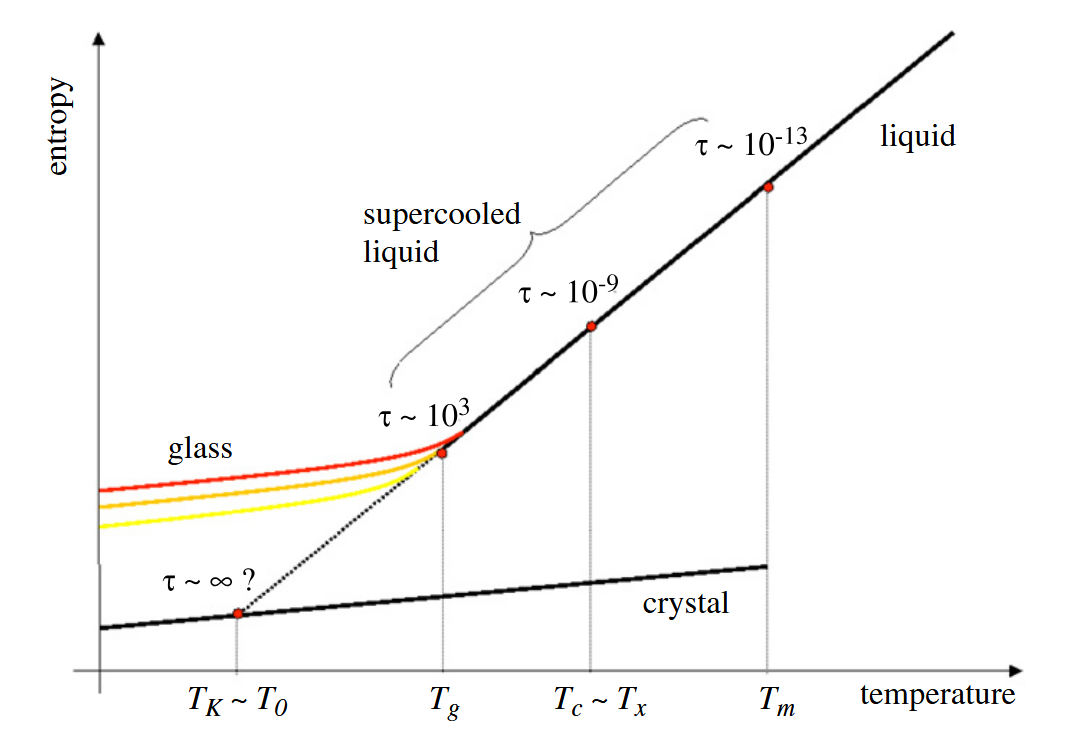
\includegraphics[width=\linewidth]{entropy_temperature_plot.png} \\[0.1cm]
				{\scriptsize\color{MutedColor} Entropia in funzione della temperatura (Cavagna, \textit{Phys. Rep.}, 2009)}
			\end{column}
		\end{columns}
	\end{frame}
	
	\begin{frame}{Andamento della viscosità ed equazione MYEGA}
		\begin{columns}[c]
			\begin{column}{0.45\textwidth}
				\centering
				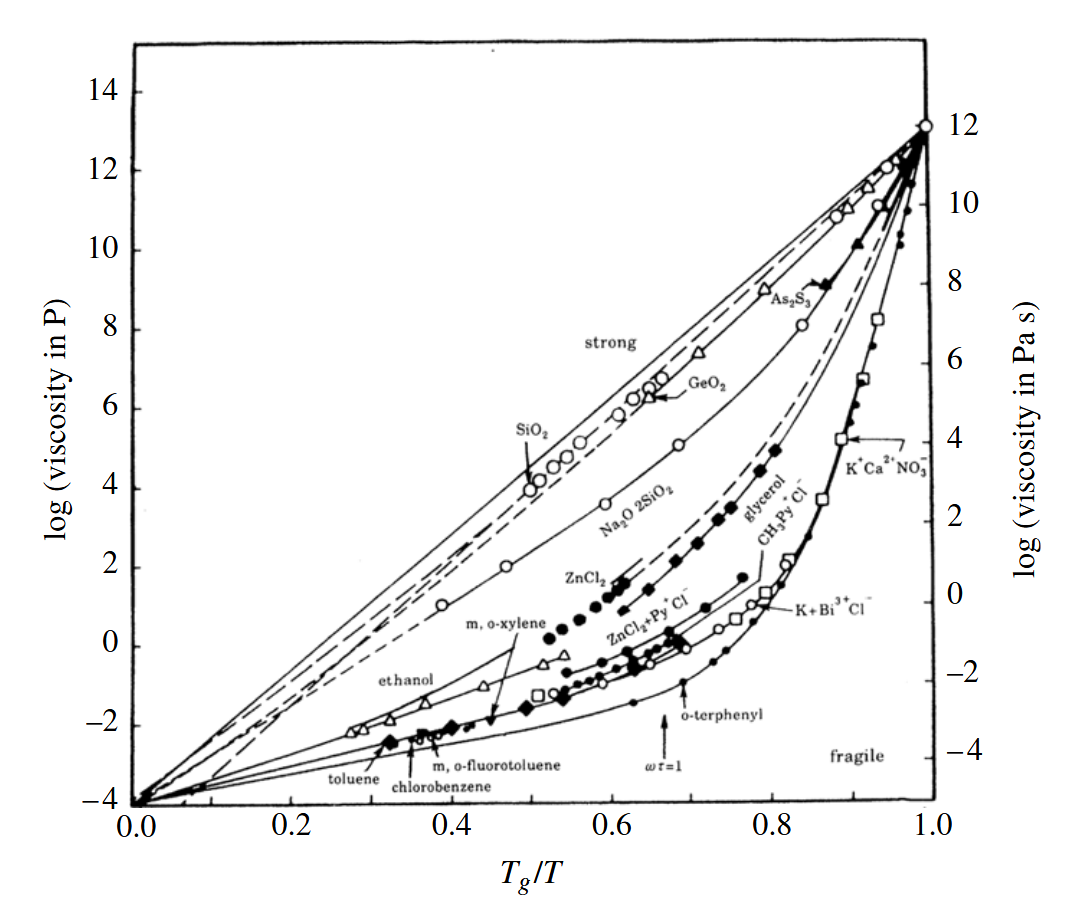
\includegraphics[height=6.2cm]{angell_plot.png} \\[0.1cm]
				{\scriptsize\color{MutedColor} Grafico di Angell (Angell, \textit{Science}, 1995)}
			\end{column}
			\hspace{0.4cm}
			\begin{column}{0.5\textwidth}
				\small
				\textbf{Legge di Arrhenius}
				\vspace{-0.2cm}
				$$\eta(T) = \eta_\infty \exp\left( \frac{E_a}{k_B T} \right)$$
				
				\vspace{0.05cm}
				\textbf{Modello MYEGA}
				\vspace{-0.2cm}
				$$\eta(T) = \eta_\infty \exp \left[ \frac{K}{T} \exp\left( \frac{C}{T} \right) \right]$$
				
				\vspace{0.05cm}
				Riscrittura in funzione di ($T_g, m, \eta_\infty$)
				\vspace{-0.2cm}
				{\footnotesize
					$$\begin{aligned}
						\log_{10} \eta(T) &= \log_{10} \eta_\infty + (12 - \log_{10} \eta_\infty) \frac{T_g}{T} \times \\
						&\times \exp \left[ \left( \frac{m}{12 - \log_{10} \eta_\infty} - 1 \right) \left( \frac{T_g}{T} - 1 \right) \right]
					\end{aligned}$$}
				
				\vspace{0.15cm}
				\begin{tikzpicture}[opacity=0]
					\node[draw=red!75!black, fill=red!6, thick, rounded corners=3pt, inner sep=6pt, text width=0.92\linewidth, align=left, font=\footnotesize] {
						\textbf{\color{red!75!black} Approccio \textit{data-driven}}\\
						Predire $(T_g, m, \eta_\infty)$ direttamente dalla composizione chimica del liquido.
					};
				\end{tikzpicture}
			\end{column}
		\end{columns}
	\end{frame}
	
	\begin{frame}[noframenumbering]{Andamento della viscosità ed equazione MYEGA}
		\begin{columns}[c]
			\begin{column}{0.45\textwidth}
				\centering
				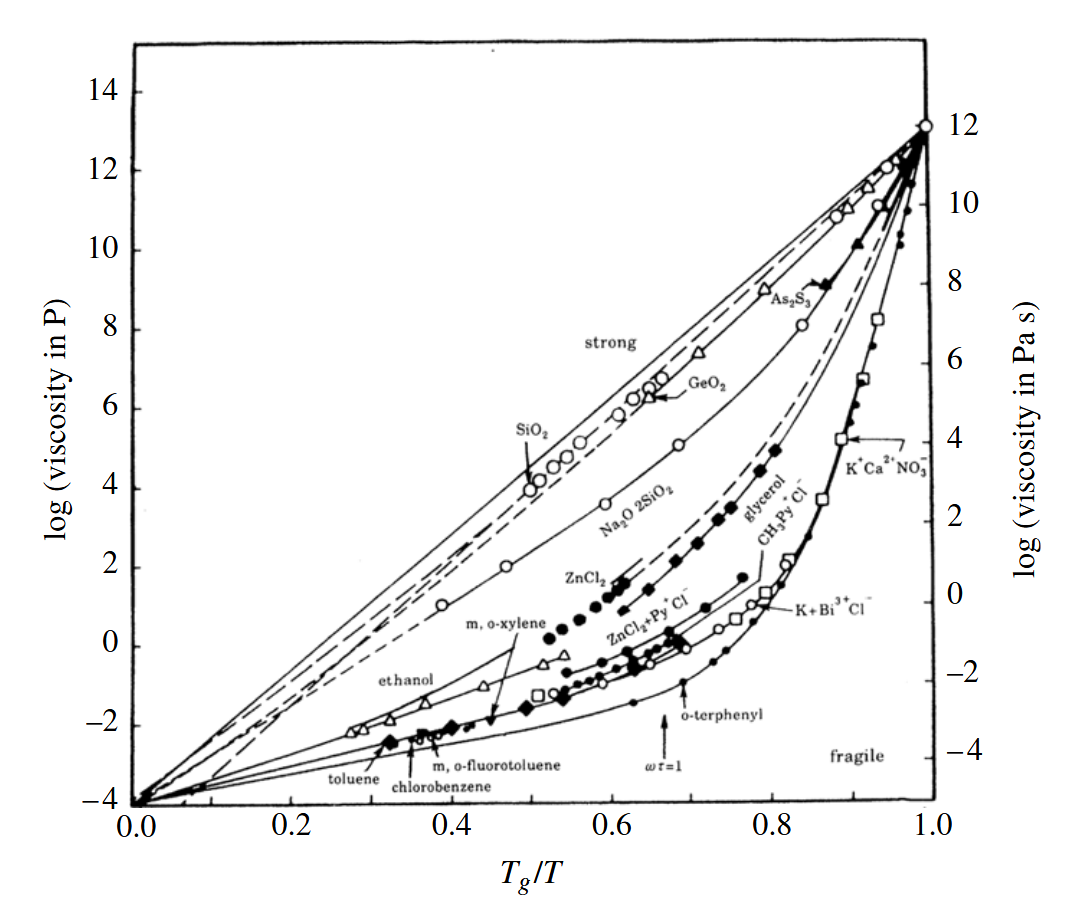
\includegraphics[height=6.2cm]{angell_plot.png} \\[0.1cm]
				{\scriptsize\color{MutedColor} Grafico di Angell (Angell, \textit{Science}, 1995)}
			\end{column}
			\hspace{0.4cm}
			\begin{column}{0.5\textwidth}
				\small
				\textbf{Legge di Arrhenius}
				\vspace{-0.2cm}
				$$\eta(T) = \eta_\infty \exp\left( \frac{E_a}{k_B T} \right)$$
				
				\vspace{0.05cm}
				\textbf{Modello MYEGA}
				\vspace{-0.2cm}
				$$\eta(T) = \eta_\infty \exp \left[ \frac{K}{T} \exp\left( \frac{C}{T} \right) \right]$$
				
				\vspace{0.05cm}
				Riscrittura in funzione di ($T_g, m, \eta_\infty$)
				\vspace{-0.2cm}
				{\footnotesize
					$$\begin{aligned}
						\log_{10} \eta(T) &= \log_{10} \eta_\infty + (12 - \log_{10} \eta_\infty) \frac{T_g}{T} \times \\
						&\times \exp \left[ \left( \frac{m}{12 - \log_{10} \eta_\infty} - 1 \right) \left( \frac{T_g}{T} - 1 \right) \right]
					\end{aligned}$$}
				
				\vspace{0.15cm}
				\begin{tikzpicture}
					\node[draw=red!75!black, fill=red!6, thick, rounded corners=3pt, inner sep=6pt, text width=0.92\linewidth, align=left, font=\footnotesize] {
						\textbf{\color{red!75!black} Approccio \textit{data-driven}}\\
						Predire $(T_g, m, \eta_\infty)$ direttamente dalla composizione chimica del liquido.
					};
				\end{tikzpicture}
			\end{column}
		\end{columns}
	\end{frame}
	
	\begin{frame}{Pipeline di lavoro di ViscNet}
		\centering
		\begin{tikzpicture}
			\node[anchor=south west, inner sep=0pt] (img) at (0,0) {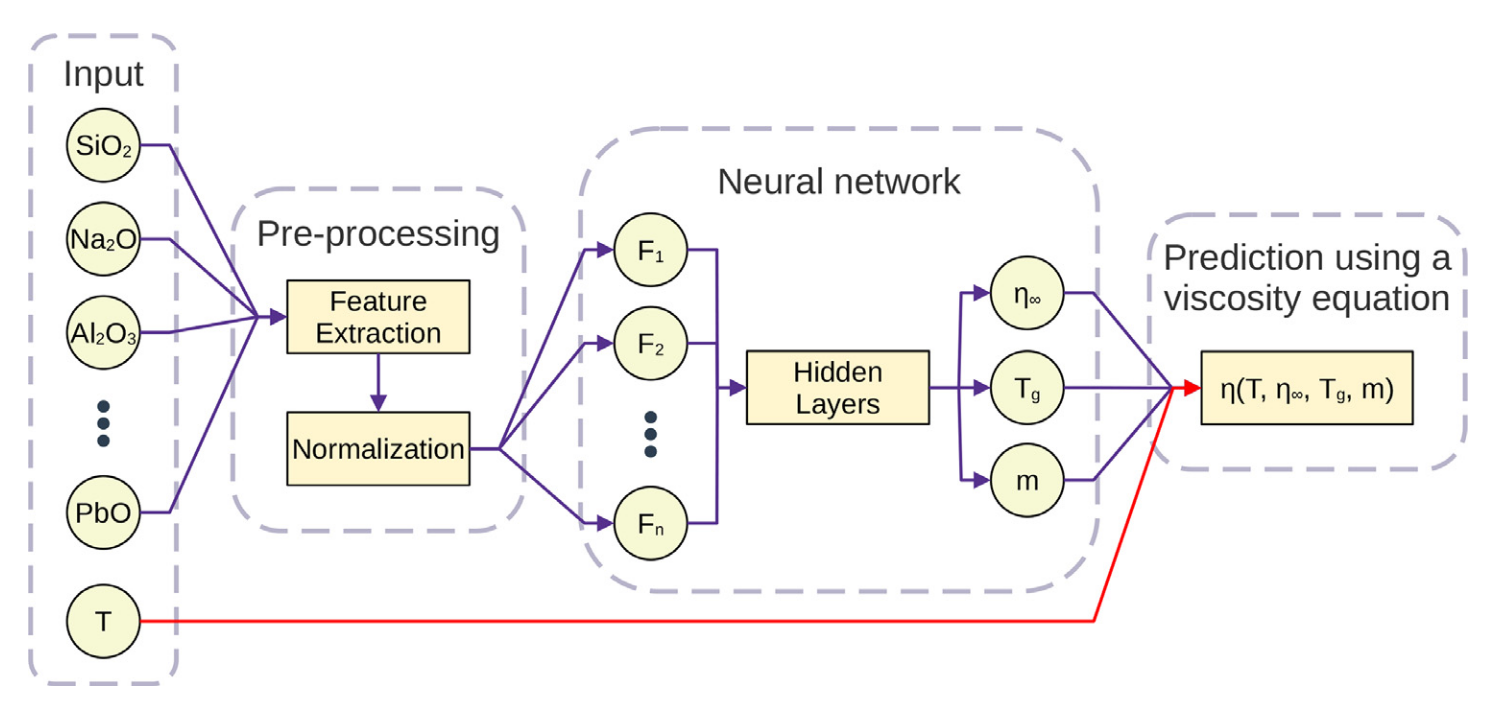
\includegraphics[width=0.78\textwidth]{flowchart_viscnet.png}};
		\end{tikzpicture} \\[0.05cm]
		{\scriptsize\color{MutedColor} Flowchart della pipeline implementata nel modello ViscNet (Cassar, \textit{Acta Materialia}, 2021)}
		
		\vspace{0.3cm}
		\begin{columns}[c]
			\begin{column}{0.5\textwidth}
				\vphantom{\small\textbf{Modello di regressione lineare:}}
			\end{column}
			\begin{column}{0.5\textwidth}
				\vphantom{\small $y = w_0 + \sum_{i=1}^M w_i x_i = w_0 + \mathbf{w}^T \mathbf{x}$}
			\end{column}
		\end{columns}
	\end{frame}
	
	\begin{frame}[noframenumbering]{Pipeline di lavoro adottata}
		\centering
		\begin{tikzpicture}
			\node[anchor=south west, inner sep=0pt] (img) at (0,0) {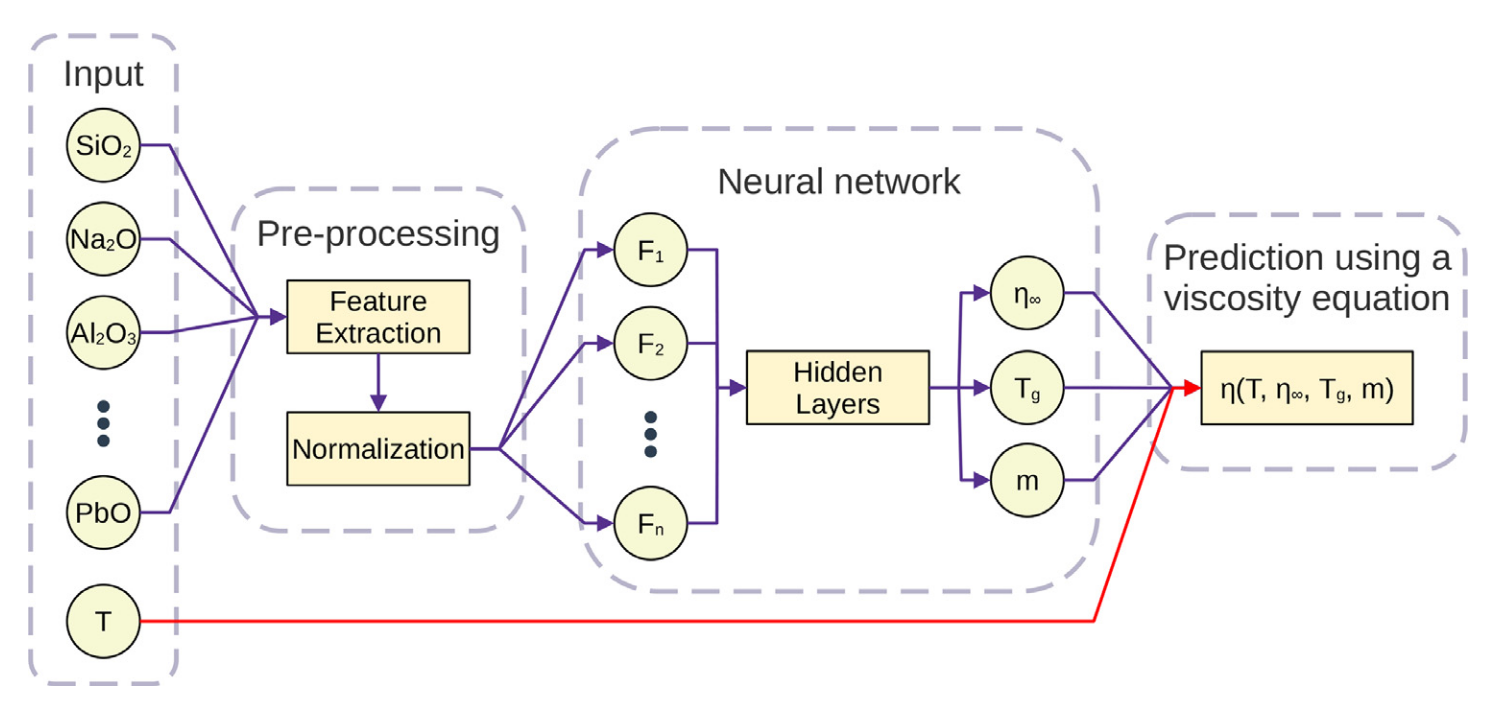
\includegraphics[width=0.78\textwidth]{flowchart_viscnet.png}};
			\begin{scope}[x={(img.south east)}, y={(img.north west)}]
				\fill[white] (0.43, 0.71) rectangle (0.70, 0.80);
				\node[font=\footnotesize\sffamily\bfseries, text=red!75!black] at (0.563, 0.75) {Linear regression};
				
				\fill[white] (0.463, 0.22) rectangle (0.663, 0.67);
				
				\foreach \yi in {0.645, 0.512, 0.259} {
					\foreach \yj in {0.582, 0.451, 0.317} {
						\draw[->, >=stealth, color=PrimaryColor!85, line width=0.6pt] (0.464, \yi) -- (0.662, \yj);
					}
				}
				
				\draw[red!75!black, line width=1.3pt, rounded corners=16pt] (0.390, 0.160) rectangle (0.735, 0.818);
			\end{scope}
		\end{tikzpicture} \\[0.05cm]
		{\scriptsize\color{MutedColor}\vphantom{Flowchart della pipeline implementata nel modello ViscNet (Cassar, \textit{Acta Materialia}, 2021)}}
		
		\vspace{0.3cm}
		\begin{columns}[c]
			\begin{column}{0.5\textwidth}
				\raggedleft
				\small\textbf{Modello di regressione lineare:}
			\end{column}
			\begin{column}{0.5\textwidth}
				\raggedright
				\small $y = w_0 + \sum_{i=1}^M w_i x_i = w_0 + \mathbf{w}^T \mathbf{x}$
			\end{column}
		\end{columns}
	\end{frame}
	
	\begin{frame}{Dataset ed estrazione delle \textit{features}}
		\begin{columns}[T]
			\begin{column}{0.46\textwidth}
				\small
				\textbf{Dati sperimentali e partizionamento}
				\vspace{0.2cm}
				\begin{itemize}
					\item Database di origine: \textbf{SciGlass} (liquidi formatori di vetro a base di ossidi)
					\vspace{0.15cm}
					\item Dataset complessivo: \textbf{847 liquidi} (\textbf{17\,584 misurazioni} di viscosità)
					\vspace{0.15cm}
					\item \textit{Training set}: \textbf{762 liquidi}
					\vspace{0.15cm}
					\item \textit{Unseen test set}: \textbf{85 liquidi}
				\end{itemize}
			\end{column}
			\begin{column}{0.50\textwidth}
				\small
				\textbf{Costruzione dei descrittori chimico-fisici}
				\vspace{0.2cm}
				
				Dalle frazioni molari atomiche $\boldsymbol{C}$ e dalle proprietà chimiche elementari $\boldsymbol{S}$:
				$$\boldsymbol{W} = \boldsymbol{C} \circ \boldsymbol{S}$$
				$$\boldsymbol{A} = \lceil \boldsymbol{C} \rceil \circ \boldsymbol{S}$$
				
				\vspace{0.2cm}
				Applicando 5 funzioni di aggregazione statistica (\textit{somma, media, deviazione standard, minimo, massimo}) si ottengono $\mathbf{M = 560}$ \textbf{\textit{features}}.
			\end{column}
		\end{columns}
	\end{frame}
	
	\begin{frame}{Gestione della multicollinearità nei modelli lineari}
		\small
		\textbf{Minimi Quadrati Ordinari (OLS)}
		$$\mathcal{L}_{\text{OLS}}(\mathbf{w}) = \frac{1}{2N}\|\mathbf{y} - X\mathbf{w}\|_2^2$$
		
		\vspace{0.25cm}
		\textbf{Ridge Regression ($L_2$)}
		$$\mathcal{L}_{\text{Ridge}}(\mathbf{w}) = \frac{1}{2N}\|\mathbf{y} - X\mathbf{w}\|_2^2 + \frac{\alpha}{2}\|\mathbf{w}\|_2^2$$
		
		\vspace{0.25cm}
		\textbf{Elastic Net ($L_1 + L_2$)}
		\vspace{-0.2cm}
		\begin{columns}[c]
			\begin{column}{0.62\textwidth}
				$$\begin{aligned}
					\mathcal{L}_{\text{EN}}(\mathbf{w}) &= \frac{1}{2N}\|\mathbf{y} - X\mathbf{w}\|_2^2 + \lambda_1 \|\mathbf{w}\|_1 + \frac{\lambda_2}{2} \|\mathbf{w}\|_2^2 \\[0.2cm]
					&= \frac{1}{2N}\|\mathbf{y} - X\mathbf{w}\|_2^2 + \alpha \left( \beta \|\mathbf{w}\|_1 + \frac{1-\beta}{2} \|\mathbf{w}\|_2^2 \right)
				\end{aligned}$$
			\end{column}
			\begin{column}{0.34\textwidth}
				$$\begin{cases}
					\alpha = \lambda_1 + \lambda_2 \\[0.2cm]
					\beta = \dfrac{\lambda_1}{\lambda_1 + \lambda_2} \in [0, 1]
				\end{cases}$$
			\end{column}
		\end{columns}
	\end{frame}
	
	\begin{frame}{Filtraggio iterativo VIF}
		\small
		$$\text{VIF}_j = \frac{1}{1 - R_j^2} \qquad \qquad R^2 = 1 - \frac{\sum_{i=1}^{N} (y_i - \hat{y}_i)^2}{\sum_{i=1}^{N} (y_i - \bar{y})^2}$$
		\vspace{0.3cm}
		\begin{itemize}
			\item \textbf{Procedura iterativa:} ad ogni ciclo si calcola il $\text{VIF}_j$ regredendo ciascuna \textit{feature} sulle restanti $M-1$ e si elimina la variabile con valore massimo se $\text{VIF}_j > 10$ ($R_j^2 > 0.90$).
			\vspace{0.25cm}
			\item \textbf{Confronto con ViscNet:} la stessa procedura è impiegato nella pipeline di pre-elaborazione di ViscNet prima dell'addestramento della rete neurale.
		\end{itemize}
	\end{frame}
	
\begin{frame}{Scelta dei parametri}
	\begin{columns}[c]
		\begin{column}{0.48\textwidth}
			\centering
			{\footnotesize\bfseries Performance su viscosità globale ($R^2$)} \\[0.15cm]
			\adjincludegraphics[trim={0cm 0cm {0.5\width} 0.8cm}, clip, height=5.6cm]{performance/ridge/Cross_validation_Ridge_Global_Viscosity_vs_Alpha.pdf} \\[0.1cm]
			{\footnotesize Parametro selezionato: $\bm{\alpha = 0.01}$}
		\end{column}
		\begin{column}{0.48\textwidth}
		\end{column}
	\end{columns}
\end{frame}

\begin{frame}[noframenumbering]{Scelta dei parametri}
	\begin{columns}[c]
		\begin{column}{0.48\textwidth}
			\centering
			{\footnotesize\bfseries Performance su viscosità globale ($R^2$)} \\[0.15cm]
			\adjincludegraphics[trim={0cm 0cm {0.5\width} 0.8cm}, clip, height=5.6cm]{performance/ridge/Cross_validation_Ridge_Global_Viscosity_vs_Alpha.pdf} \\[0.1cm]
			{\footnotesize Parametro selezionato: $\bm{\alpha = 0.01}$}
		\end{column}
		\begin{column}{0.48\textwidth}
			\centering
			{\footnotesize\bfseries Cross-Validation a 5 fold ($R^2$)} \\[0.15cm]
			\adjincludegraphics[trim={0.2cm 0.3cm {0.5\width} 1.5cm}, clip, height=5.3cm]{performance/elastic_net/ElasticNet_CV_Heatmap_Global_Viscosity.pdf} \\[0.2cm]
			{\footnotesize Parametri selezionati: $\bm{\alpha = 0.1,\; \beta = 0.8}$}
		\end{column}
	\end{columns}
\end{frame}
	
	\begin{frame}{Valutazione delle performance predittive}
		\footnotesize
		\centering
		\renewcommand{\arraystretch}{1.25}
		\begin{tabular}{l|c|c|c|c}
			\toprule
			& \textbf{Viscosità Globale} & \textbf{Target: $T_g$} & \textbf{Target: $m$} & \textbf{Target: $\log_{10}\eta_\infty$} \\
			\textbf{Modello} & $\bm{R^2}$ & $\bm{R^2}$ & $\bm{R^2}$ & $\bm{R^2}$ \\
			\midrule
			Ridge ($\alpha = 0.01$) & 0.935 & 0.896 & 0.771 & 0.220 \\
			Elastic Net ($\alpha=0.1;\,\beta=0.8$) & 0.806 & 0.778 & 0.712 & 0.162 \\
			VIF + OLS & 0.776 & 0.819 & 0.761 & 0.200 \\
			\bottomrule
		\end{tabular}
		
		\vspace{0.6cm}
		\begin{tabular}{lcccc}
			\toprule
			\textbf{Modello} & $\bm{R^2}$ ($\uparrow$) & \textbf{RMSE} ($\downarrow$) & \textbf{MAE} ($\downarrow$) & \textbf{MedAE} ($\downarrow$) \\
			\midrule
			ViscNet & 0.926 & 1.100 & 0.780 & 0.530 \\
			\textbf{Ridge Regression} & \textbf{0.935} & \textbf{1.031} & \textbf{0.657} & \textbf{0.392} \\
			\bottomrule
		\end{tabular}
	\end{frame}
	
	\begin{frame}{Qualità dell'interpolazione}
		\begin{columns}[c]
			\begin{column}{0.48\textwidth}
				\centering
				{\footnotesize\bfseries Ridge Regression} \\[0.1cm]
				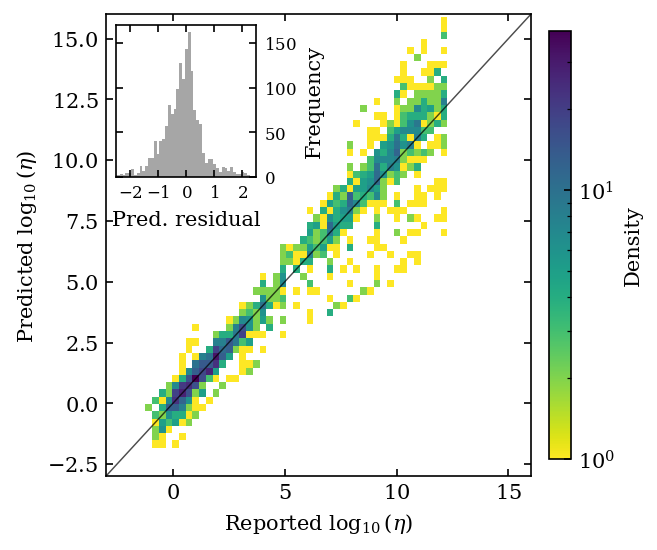
\includegraphics[height=5.5cm]{correlazione/ridge_2D_density_histogram.png} \\
				{\scriptsize\color{MutedColor}\vphantom{(Cassar, \textit{Acta Materialia}, 2021)}}
			\end{column}
			\begin{column}{0.48\textwidth}
				\centering
				{\footnotesize\bfseries ViscNet} \\ [0.1cm]
				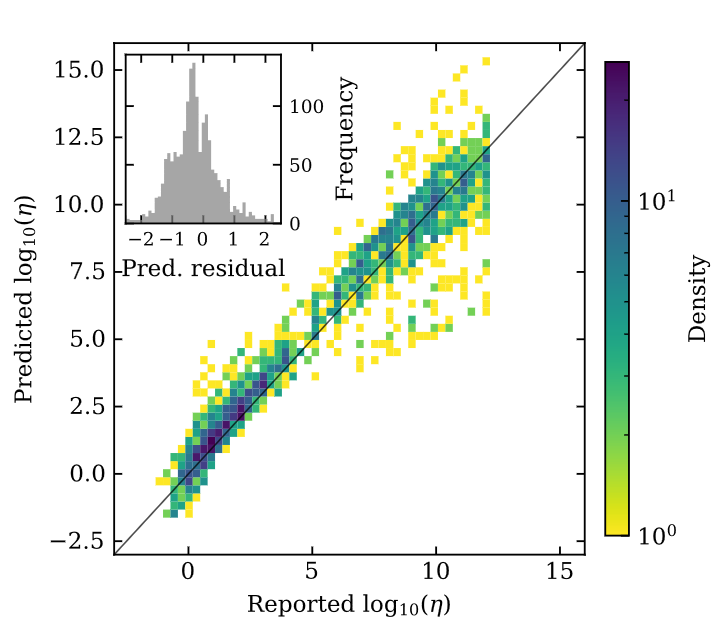
\includegraphics[trim={0cm 0cm 0cm 0.5cm}, clip, height=5.5cm]{correlazione_viscnet.png}
				{\scriptsize\color{MutedColor} (Cassar, \textit{Acta Materialia}, 2021)}
			\end{column}
		\end{columns}
	\end{frame}
	
	\begin{frame}{Incertezza dei dati e distanza chimica}
		\begin{columns}[c]
			\begin{column}{0.48\textwidth}
				\centering
				{\footnotesize\bfseries Sovrapposizione sperimentale (ID 155)} \\[0.15cm]
				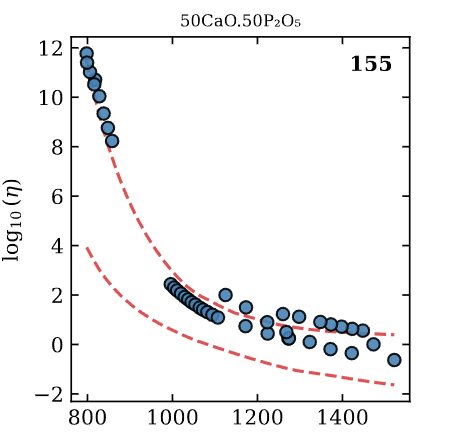
\includegraphics[trim=0cm 0cm 0cm 0.1cm, clip, height=5.2cm]{test_viscosity_plots/ridge/data_merging.png}
			\end{column}
			\begin{column}{0.48\textwidth}
				\centering
				{\\[0.01cm] \footnotesize\bfseries Errore in funzione della composizione chimica} \\[0.3cm]
				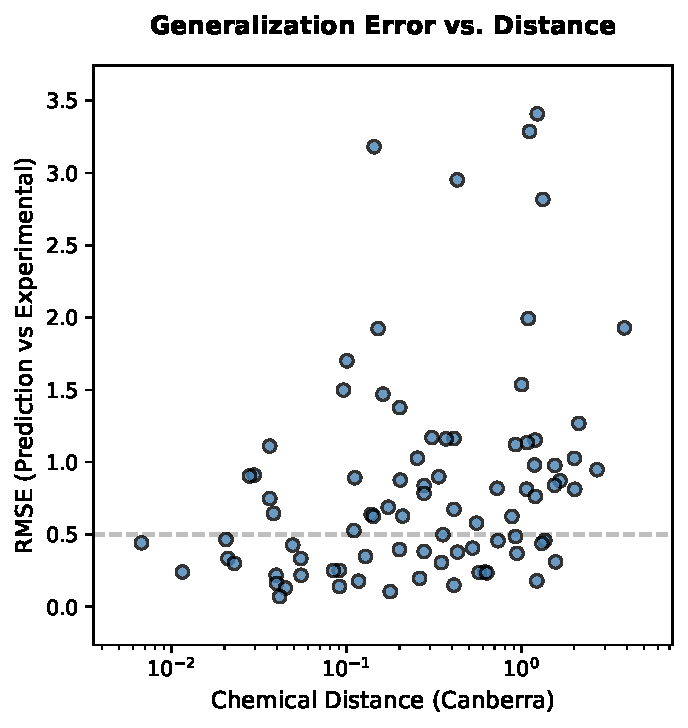
\includegraphics[trim=0cm 0cm 0cm 0.7cm, clip, height=5.2cm]{distanza/ridge_distance_plot.pdf}
			\end{column}
		\end{columns}
	\end{frame}
	
	\begin{frame}{Distribuzione dei pesi per $T_g$}
		\begin{columns}[c]
			\begin{column}{0.32\textwidth}
				\centering
				{\footnotesize\bfseries Ridge Regression} \\[0.15cm]
				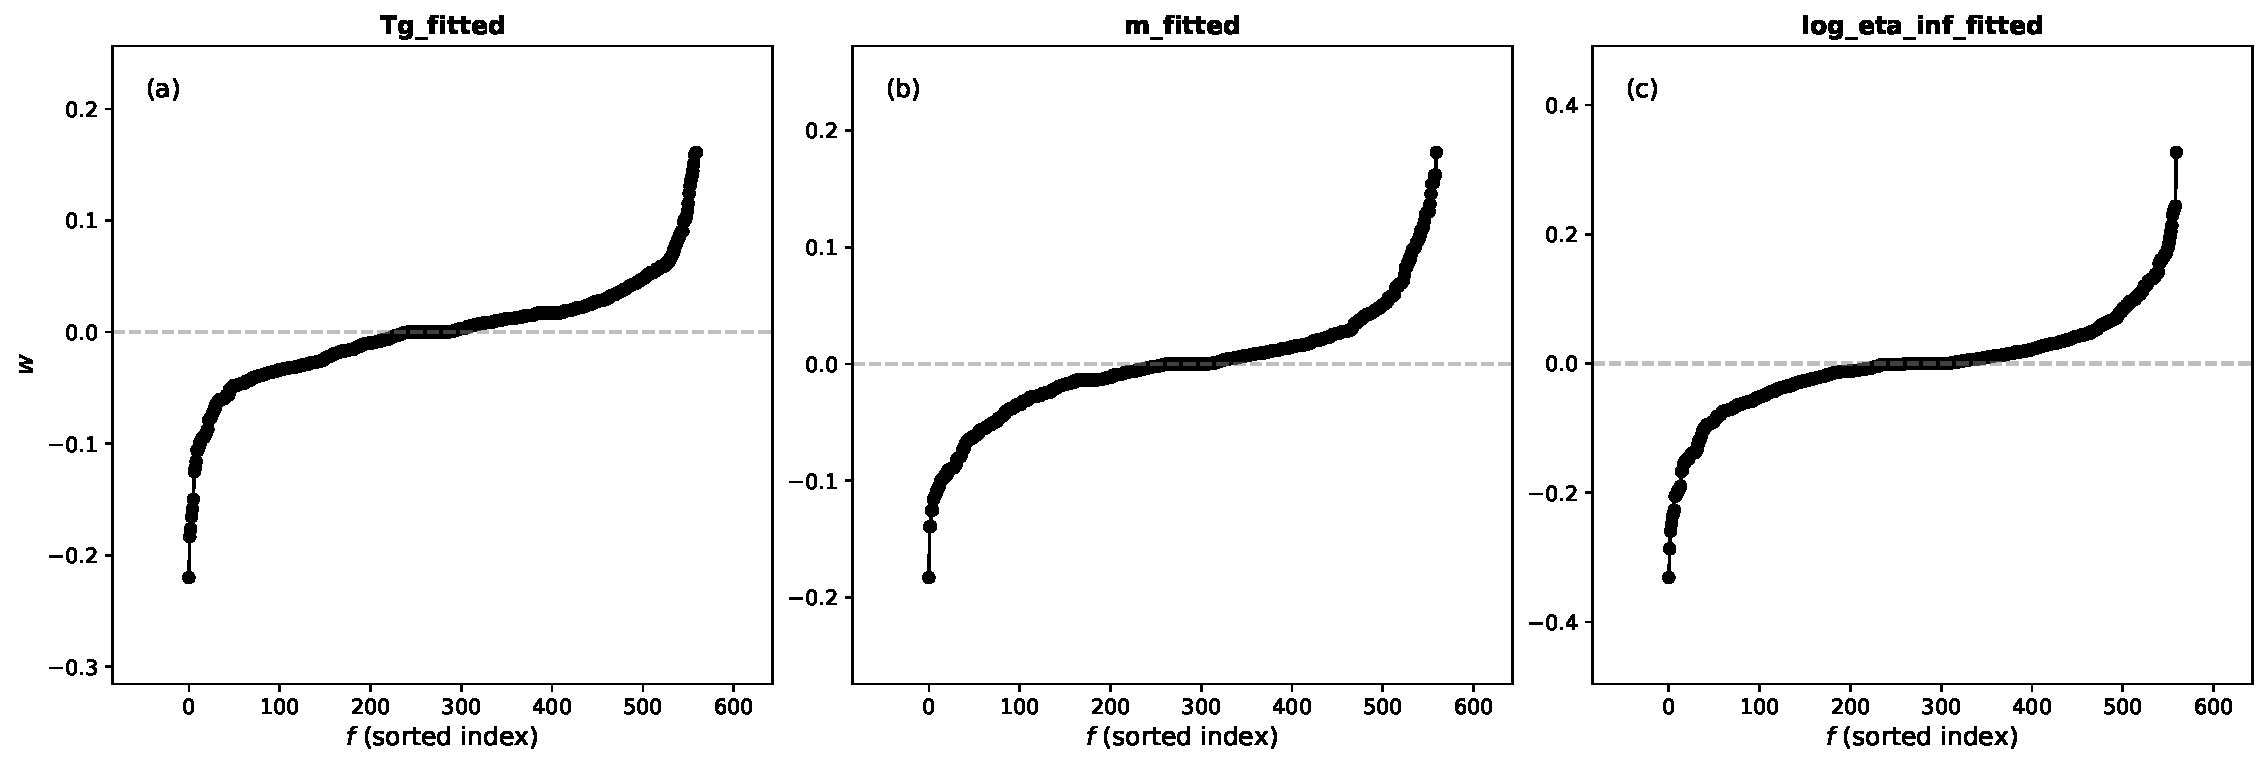
\includegraphics[trim=0.7cm 0cm 25cm 0.7cm, clip, width=\linewidth]{importanza_features/ridge_features_importance.pdf}
			\end{column}
			\begin{column}{0.32\textwidth}
				\centering
				{\footnotesize\bfseries VIF + OLS} \\[0.15cm]
				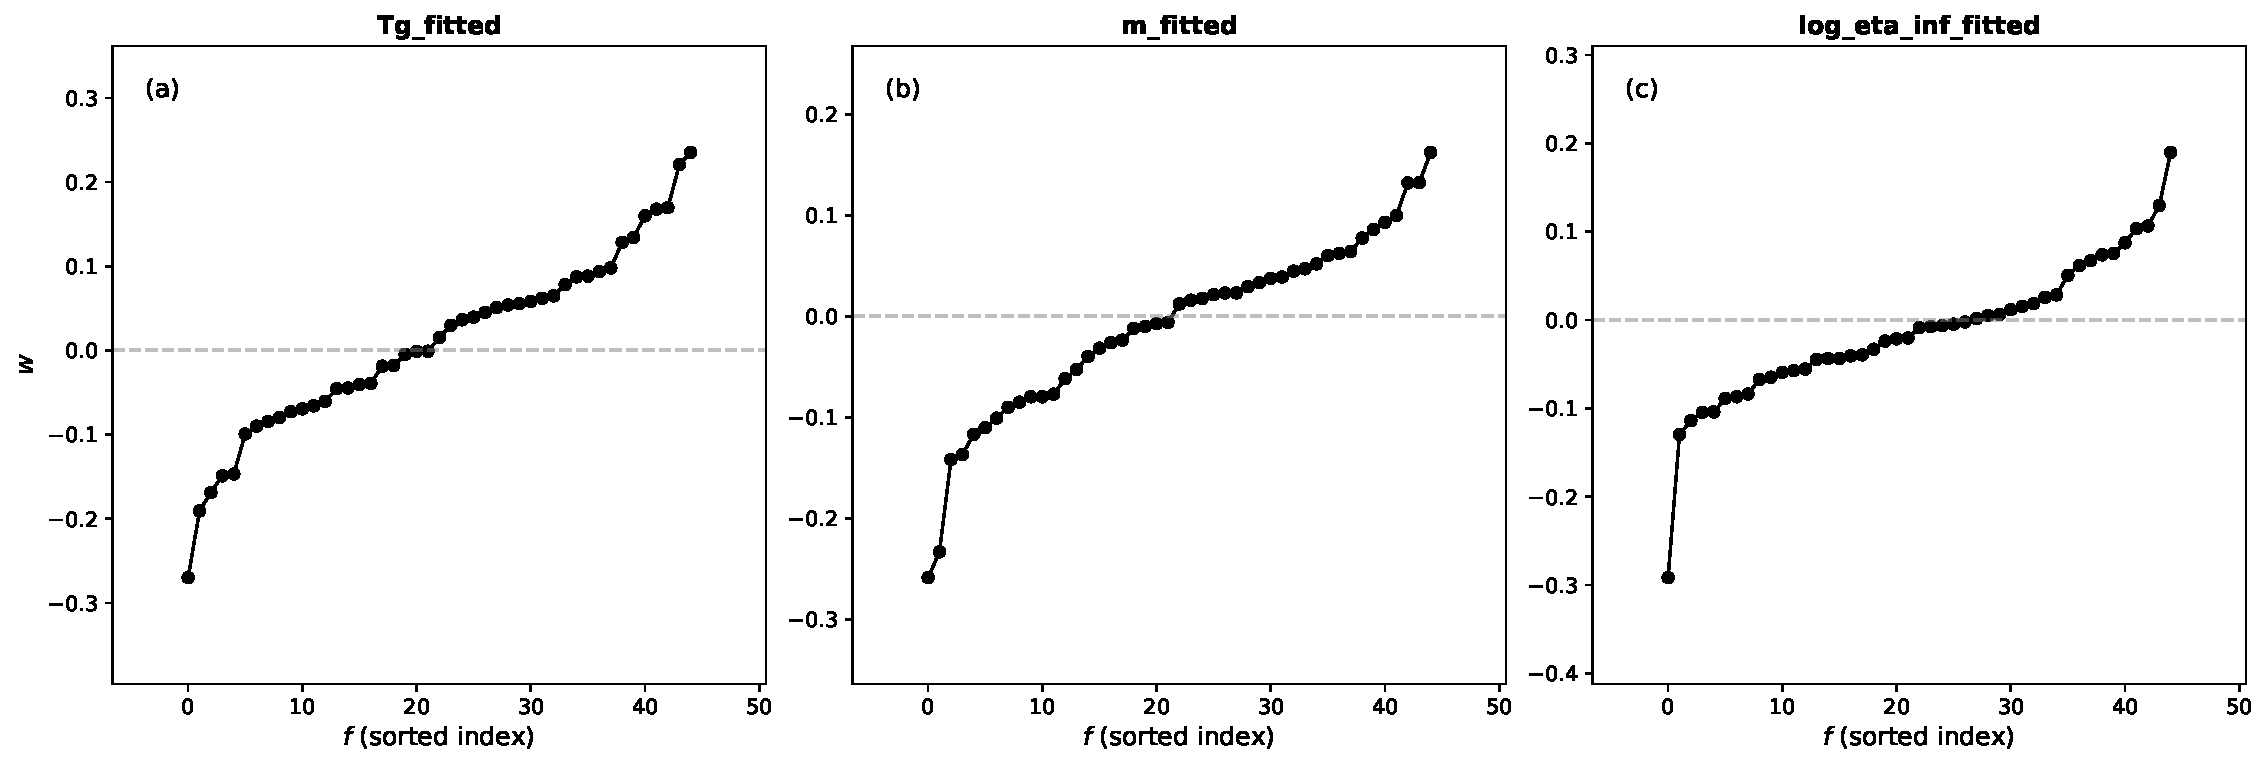
\includegraphics[trim=0.7cm 0cm 25cm 0.7cm, clip, width=\linewidth]{importanza_features/vif_ols_features_importance.pdf}
			\end{column}
			\begin{column}{0.32\textwidth}
				\centering
				{\footnotesize\bfseries Elastic Net} \\[0.15cm]
				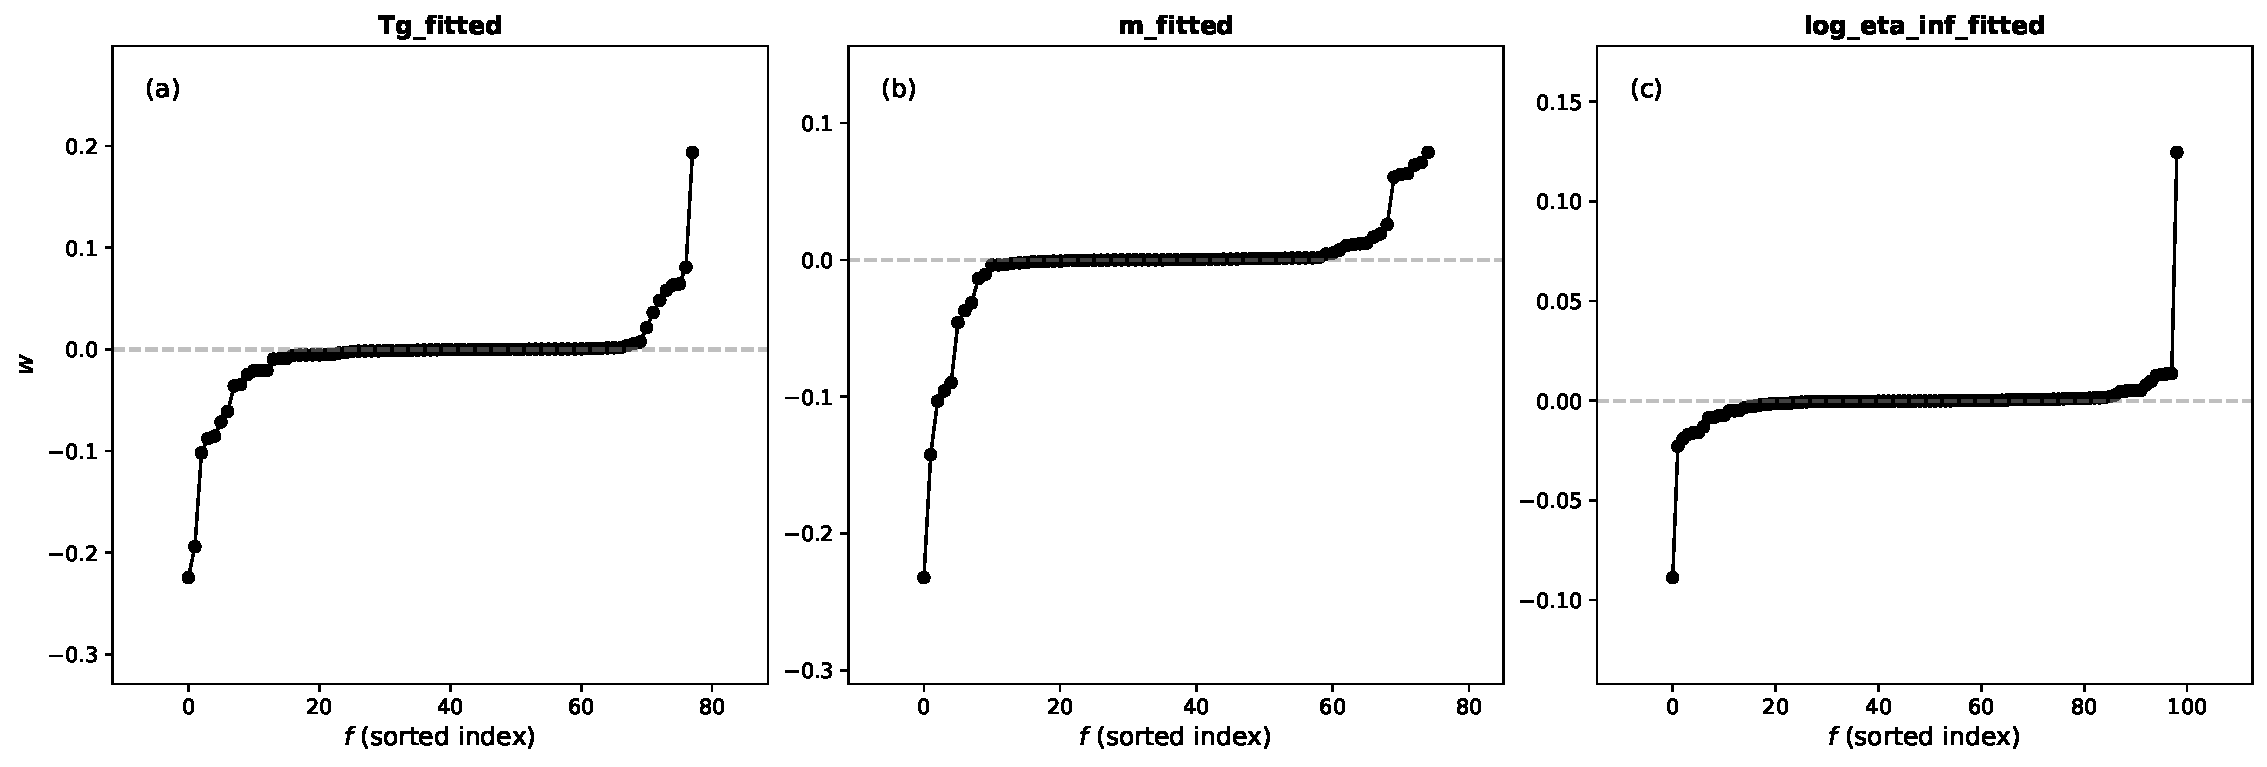
\includegraphics[trim=0.7cm 0cm 25cm 0.7cm, clip, width=\linewidth]{importanza_features/elastic_net_features_importance_no_zeroes.pdf}
			\end{column}
		\end{columns}
	\end{frame}
	
	\begin{frame}{Analisi dei pesi principali per $T_g$ (Elastic Net)}
		\centering
		\footnotesize
		\renewcommand{\arraystretch}{1.2}
		\begin{tabular}{cl r}
			\toprule
			\textbf{Rank} & \textbf{Feature} & \textbf{Peso} \\
			\midrule
			1 & \texttt{W\_Sum\_GSbandgap} & $-0.224$ \\
			\rowcolor{HighlightBg} 2 & \texttt{W\_Sum\_NsUnfilled} & $-0.194$ \\
			\rowcolor{HighlightBg} 3 & \texttt{W\_Sum\_NsValence} & $0.194$ \\
			4 & \texttt{W\_Std\_density} & $-0.102$ \\
			5 & \texttt{W\_Max\_GSbandgap} & $-0.088$ \\
			6 & \texttt{A\_Std\_zeff} & $-0.085$ \\
			7 & \texttt{A\_Max\_vdw\_radius\_uff} & $0.081$ \\
			8 & \texttt{A\_Max\_zeff} & $-0.071$ \\
			9 & \texttt{A\_Max\_FusionEnthalpy} & $0.064$ \\
			10 & \texttt{A\_Max\_NpUnfilled} & $0.063$ \\
			\bottomrule
		\end{tabular}
	\end{frame}
	
	\begin{frame}{Interpretabilità dei modelli lineari}
		\small
		\begin{itemize}
			
			\item \textbf{Ridge:} conserva l'intero spazio delle 560 \textit{features} raggiungendo le prestazioni più elevate ($R^2 = 0.935$), ma produce una distribuzione continua dei pesi priva di poche variabili dominanti (``scatola nera lineare'').
			\vspace{0.35cm}
			
			\item \textbf{Elastic Net:} seleziona descrittori fisicamente coerenti (\textit{bandgap}, raggio di Van der Waals, entalpia di fusione), ma comporta un calo di accuratezza ($R^2 = 0.806$) e mantiene compensazioni matematiche tra variabili correlate.
			\vspace{0.35cm}
						
			\item \textbf{VIF + OLS:} la riduzione delle \textit{features} collineari stabilizza la stima OLS, ma la distribuzione dei pesi rimane continua senza indicare variabili più importanti delle altre.
			
		\end{itemize}
	\end{frame}
	
	\begin{frame}{Conclusioni}
		\small
		\begin{itemize}
			\item \textbf{Accuratezza:} sfruttando l'intero insieme di 560 \textit{features} regolarizzate tramite norma $L_2$, la regressione lineare Ridge supera la rete neurale ViscNet ($R^2 = 0.935$ vs $0.926$, $\text{RMSE} = 1.031$, $\text{MedAE} = 0.392$) ed evita il \textit{bias} di sovrastima a basse viscosità.
			\vspace{0.35cm}
			
			\item \textbf{Perdita di interpretabilità nei sistemi complessi:} l'impossibilità di isolare un set ristretto di descrittori senza degradare le performance sembra essere indipendente dal modello adottato e conseguenza dalla natura cooperativa della transizione vetrosa.
			\vspace{0.35cm}
			
			\item \textbf{Vantaggi della regressione lineare:} a parità di accuratezza con le reti neurali, il modello lineare offre un addestramento immediato e definisce una mappa globale e costante delle correlazioni termodinamiche.
		\end{itemize}
	\end{frame}
	
	\appendix
	
	
	\begin{frame}{Backup: Tracce Ridge e stabilità dei pesi ($T_g$)}
		\centering
		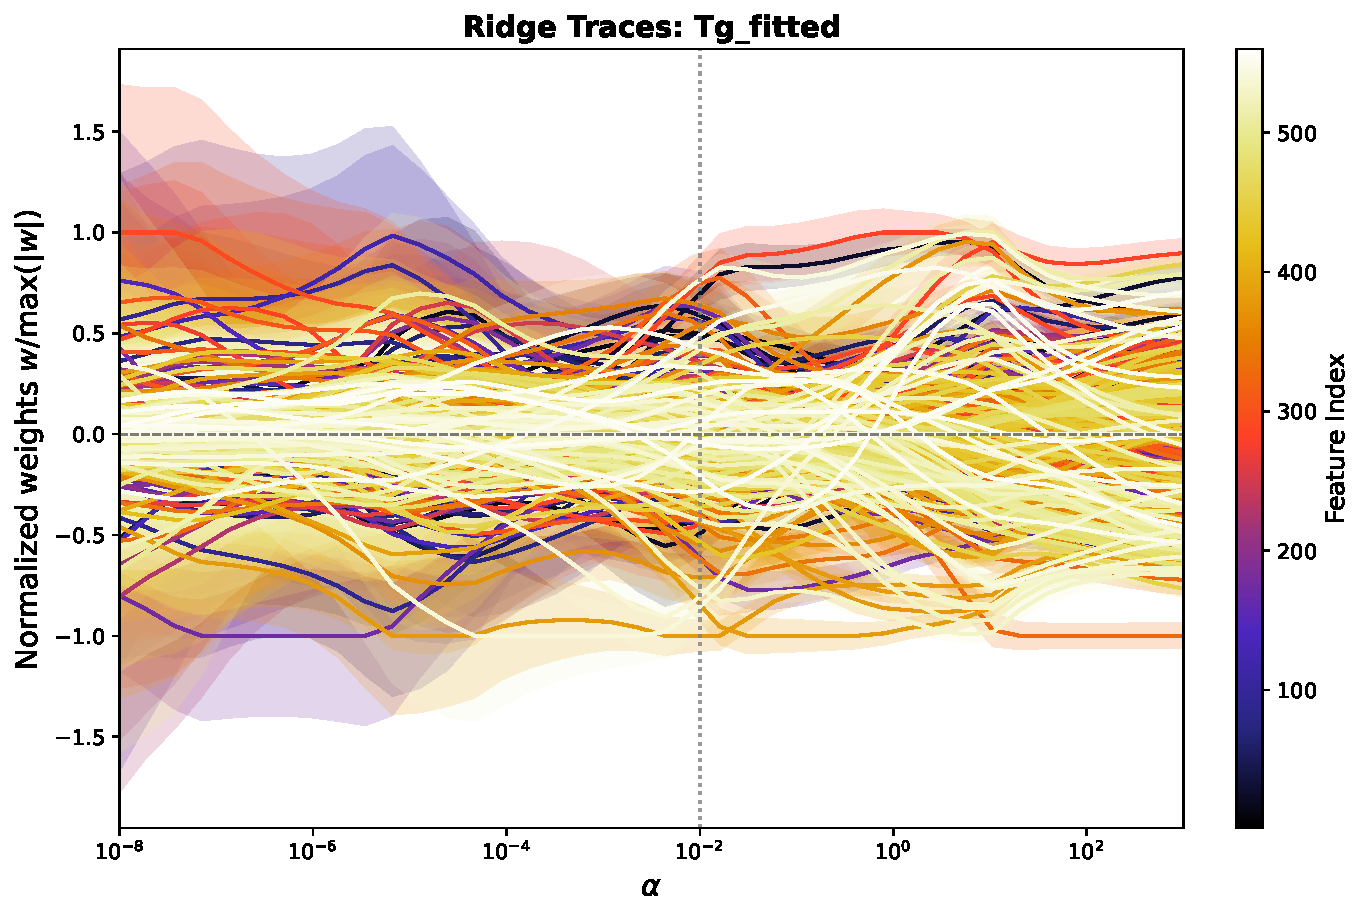
\includegraphics[trim=0cm 0cm 0cm 0.8cm, clip, height=5.6cm]{tracce_ridge/Tg_fitted.pdf} \\[0.25cm]
		\begin{minipage}{0.82\textwidth}
			\centering\footnotesize
			\textbf{Statistica su 20 \textit{split} casuali:} le linee continue indicano la media dei pesi normalizzati, \\ le bande sfumate rappresentano l'intervallo di una deviazione standard.
		\end{minipage}
	\end{frame}
	
	\begin{frame}{Backup: Regressione su Componenti Principali (PCR e SPCR)}
		\small
		Diagonalizzazione della matrice di correlazione empirica $C = \frac{1}{N_s}X^T X$:
		$$C = U \Lambda U^T \qquad \implies \qquad \tilde{X}^{(f)} = \frac{(X U)^{(f)}}{\sqrt{\lambda^{(f)}}}$$
		
		Regressione lineare su un sottospazio di $P \ll M$ componenti ortogonali:
		$$\hat{y} = \sum_{f=1}^{P} R[\tilde{X}^{(f)}, y] \tilde{X}^{(f)}$$
		
		\vspace{0.2cm}
		\begin{itemize}
			\item \textbf{PCR classica (non supervisionata):} trattiene le prime $P$ componenti ordinate per varianza strutturale spiegata ($\lambda^{(f)}$ decrescente).
			\vspace{0.2cm}
			\item \textbf{Supervised PCR (SPCR):} ordina e seleziona le $P$ componenti in base al valore assoluto della correlazione di Pearson con ciascun target $|R[\tilde{X}^{(f)}, y]|$.
		\end{itemize}
	\end{frame}
	
	\begin{frame}{Backup: Scelta di $P$ e performance (PCR vs SPCR)}
		\begin{columns}[c]
			\begin{column}{0.46\textwidth}
				\centering
				{\footnotesize\bfseries PCR ($P = 14$)} \\[0.1cm]
				\adjincludegraphics[trim={0cm 0cm {0.5\width} 0.8cm}, clip, height=3.8cm]{performance/pcr/PCR_Global_Viscosity_Performance.pdf}
			\end{column}
			\begin{column}{0.46\textwidth}
				\centering
				{\footnotesize\bfseries Supervised PCR ($P = 12$)} \\[0.1cm]
				\adjincludegraphics[trim={0cm 0cm {0.5\width} 0.8cm}, clip, height=3.8cm]{performance/spcr/SPCR_Global_Viscosity_Performance.pdf}
			\end{column}
		\end{columns}
		
		\vspace{0.25cm}
		\scriptsize
		\centering
		\renewcommand{\arraystretch}{1.15}
		\begin{tabular}{l|cc|c|c|c}
			\toprule
			& \multicolumn{2}{c|}{\textbf{Viscosità Globale}} & \textbf{Target: $T_g$} & \textbf{Target: $m$} & \textbf{Target: $\log_{10}\eta_\infty$} \\
			\textbf{Modello} & $\bm{R^2}$ & \textbf{RMSE} & $\bm{R^2}$ & $\bm{R^2}$ & $\bm{R^2}$ \\
			\midrule
			Ridge ($\alpha = 0.01$) & 0.935 & 1.031 & 0.896 & 0.771 & 0.220 \\
			SPCR ($P = 12$) & 0.798 & 1.825 & 0.773 & 0.731 & 0.283 \\
			PCR ($P = 14$) & 0.655 & 2.383 & 0.713 & 0.731 & 0.134 \\
			\bottomrule
		\end{tabular}
	\end{frame}
	
	\begin{frame}{Backup: Proiezione dei pesi nella Supervised PCR ($P=12$)}
		\centering
		{\footnotesize\bfseries Pesi nello spazio delle Componenti Principali ($T_g$, $m$, $\log_{10}\eta_\infty$)} \\[0.05cm]
		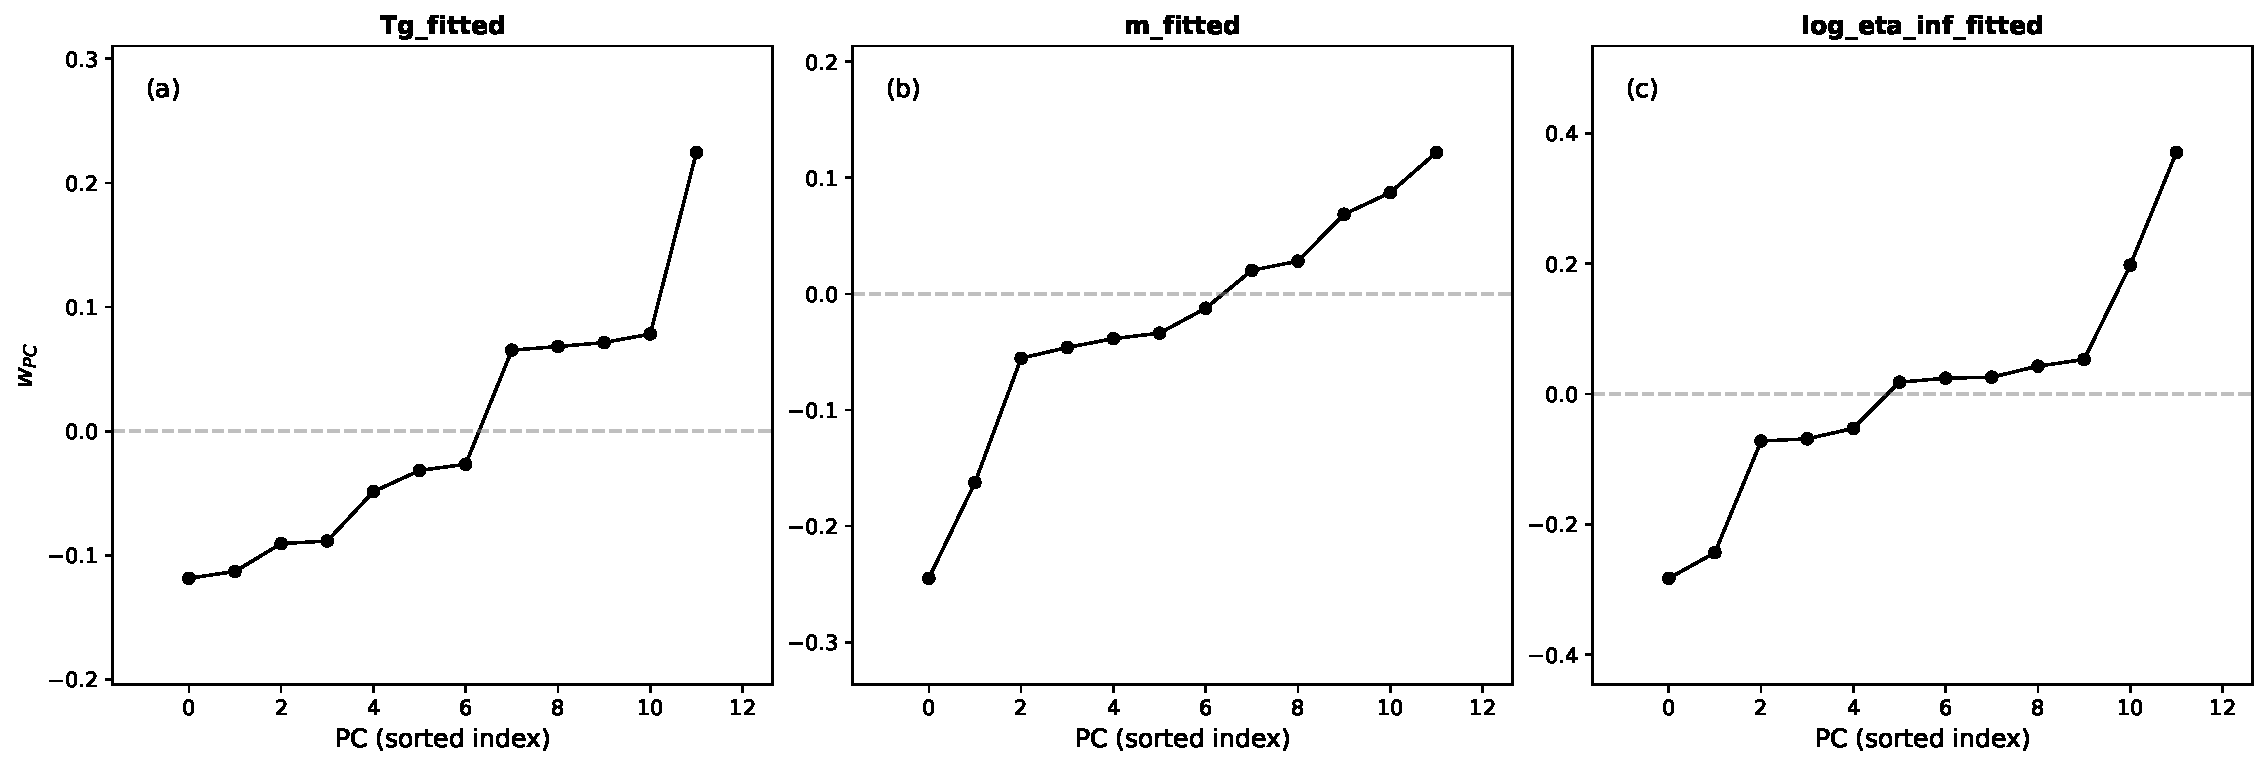
\includegraphics[trim=0cm 0cm 0cm 0.7cm, clip, width=0.68\textwidth]{importanza_features/spcr_features_importance.pdf}
		
		\vspace{0.15cm}
		{\footnotesize\bfseries Proiezione a ritroso dei pesi nello spazio delle 560 \textit{features} iniziali} \\[0.05cm]
		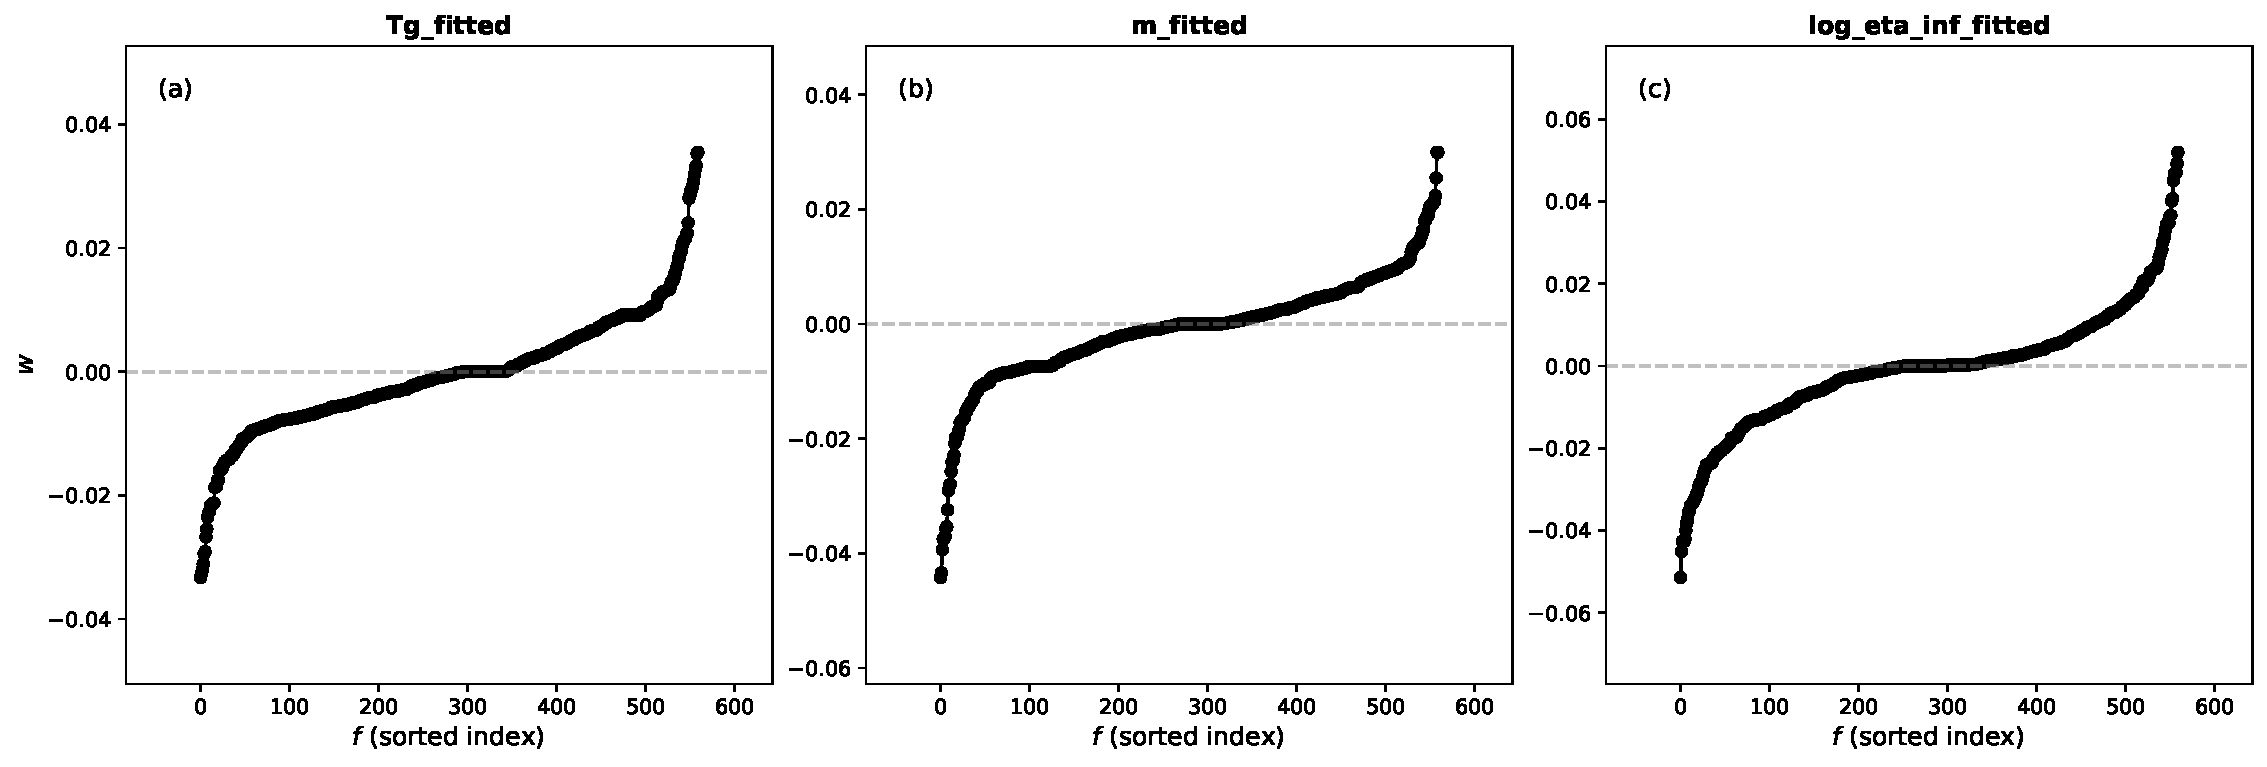
\includegraphics[trim=0cm 0cm 0cm 0.7cm, clip, width=0.68\textwidth]{importanza_features/spcr_projected_features_importance.pdf}
	\end{frame}
	
\end{document}